\documentclass[10pt,a4paper]{article}
\usepackage[utf8]{inputenc}
\usepackage[italian]{babel}
\usepackage{amsmath}
\usepackage{amsfonts}
\usepackage{amssymb}
\usepackage{graphicx}
\usepackage[left=2cm,right=2cm,top=2cm,bottom=2cm]{geometry}
\newcommand{\rem}[1]{[\emph{#1}]}

\author{Gruppo AC \\ Federico Belliardo, Giulia Franchi, Francesco Mazzoncini}
\title{Esercitazione N.7: Usi non lineari dell’ OpAmp}
\begin{document}

\maketitle
Questa esperienza ha come obbiettivo quello di studiare il funzionamento di un amplificatore operazionale modello TL081 in circuiti non lineari.

\section*{A. Discriminatore}

Si è montato il circuito in figura\ref{circuito1}, utilizzando $V_{CC} = /pm V$ e $V_{EE} = /pm V$ come tensioni di alimentazione.

\begin{figure}[h]
\centering
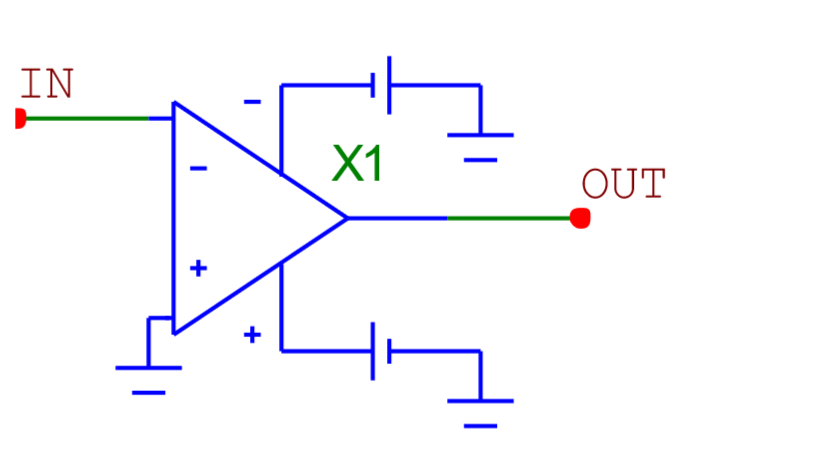
\includegraphics[scale=0.5]{Discriminatore.png}
\caption{Discriminatore realizzato con un OpAmp modello TL081.\label{circuito1}}
\end{figure}

Si è poi proseguito con lo studio della risposta del circuito ad un segnale sinusoidale. Il circuito ideale dovrebbe funzionare come un comparatore. Se così fosse, il segnale in ingresso verrebbe invertito e amplificato e l'amplificatore, a causa del grande guadagno dell'operazionale, andrebbe in saturazione restituendo un segnale uguale alla tensione di alimentazione ( $V_{EE}$ per un segnale positivo e $V_{CC}$ per uno negativo).\\
Purtroppo il circuito da noi analizzato è un amplificatore ideale e come tale presenta dei limiti al suo funzionamento.\\
Come primo limite vediamo l'influenza della tensione di offset $V_{OS}$.\\
Inoltre all'aumentare della frequenza si notano gli effetti dello slew rate finito dell'OpAmp. (come si trasforma l'onda quadra, frequenza limite per cui diventa triangolare, ecc...)
Infine, utilizzando un segnale ridotto di ampiezza, a basse frequenze comportamento ideale; ad alte frequenze clipping superiore e onda sinusoidale nella parte inferiore. Cause di tutto: finitezza del prodotto banda guadagno e la presenza di una tensione di offset negativa sul segnale del generatore di funzioni.\\

\section*{B. Amplificatore di carica}

Si è montato il circuito in figura\ref{circuito2} utilizzando i componenti $C_T = /pm nF$, $C_F = /pm nF$, $C_1 = /pm nF$, $R_1 = /pm k \Omega$, $R_2 = /pm \Omega$, $R_3 = /pm k \Omega$ e le tensioni $V_{CC} = /pm V$ e $V_{EE} = /pm V$. Si è poi regolato il potenziometro $R_3$ in modo che la tensione di soglia del discriminatore fosse ($\sim 200mV$) $V_{R3} = /pm V$ e si è fornita dal generatore di funzioni un'onda quadra.\\
\begin{figure}[h]
\centering
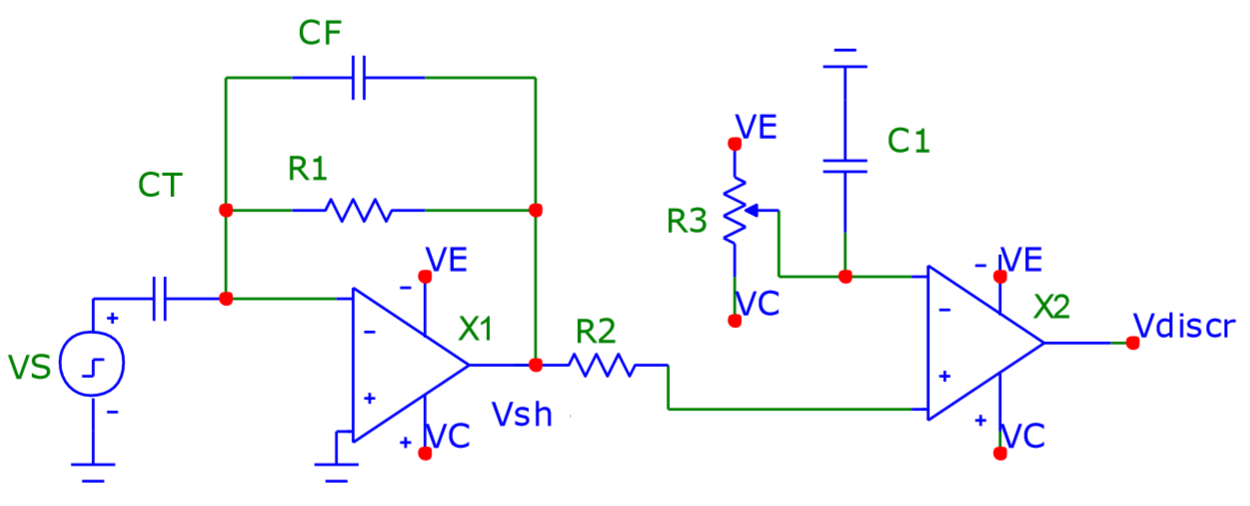
\includegraphics[scale=0.5]{amplificatoreCarica.png}
\caption{Amplificatore di carica realizzato con un OpAmp modello TL081.\label{circuito2}}
\end{figure}

\subsection*{1. Descrizione del circuito e prime misure}
Il circuito da noi montato è costituito da tre parti distinte: un circuito di iniezione di carica ($V_S$+$C_T$), un circuito formatore che converte la carica in un segnale di forma fissata (X1) e un discriminatore che confronta il circuito con una soglia prefissata (X2).


La prima parte è costituita dal generatore di forme d'onda $V_S$ e dal condensatore $C_T$, dove viene fornita una carica pari a $Q_{IN}=V_S C_T$. Il formatore invece è rappresentato dal parallelodi $C_F$ e $R_1$, all'uscita di tale circuito si ha un segnale:\\
\begin{center}
$V_{SH}=\frac{Q_{IN}}{C_F} e^{-\frac{t}{\tau}} = V_S \frac{C_T}{C_F} e^{t/R_1 C_F}$\\
\end{center}

Il resto del circuito rappresenta il discriminatore, analogo a quello descritto al punto A, ma con una tensione di soglia. I componenti $R_2$ e $C_1$ hanno il compito di disaccoppiare il circuito formatore da quello discriminatore e di ridurre il rumore sulla tensione di soglia ad alte frequenze.\\
A frequenza fissata $f = /pm Hz$ si è misurata la risposta del circuito ad un segnale di ampiezza (picco_picco o no?!) $V_S = /pm V$.\\
L'ampiezza massima attesa per il segnale $V_{SH}$, secondo la formula sopra citata, è $V_{SH,MAX,ATT} = V_S \frac{C_T}{C_F} =  /pm V$, mentre il valore misurato sperimentalmente è $V_{SH,MAX} = /pm V$.
Si è inoltre misurata l'ampiezza del segnale $V_{discr} = /pm V$.

\subsection*{2. Dipendenza del segnale in uscita dall'ampiezza del segnale in ingresso}

Sempre mantenendo una frequenza fissa $F = /pm Hz$, si è misurata, al variare dell'ampiezza, la durata nel tempo del segnale in uscita dal discriminatore, i dati sono riportati in tabella.\\

Sapendo che $V_-=V_S \frac{C_T}{C_F} e^{- \Delta t/R_1 C_F}$, si ottiene $\Delta t = -R_1 C_F log\left( \frac{V_- C_F}{V_S C_T}\right)$, dalla quale si ricava la relazione:
\begin{center}
$\Delta t = R_1 C_F log(V_S) + R_1 C_f log\left( \frac{C_T}{V_- C_F}\right)$
\end{center}

\rem{Analisi dati}

\section*{C. Trigger di Schmitt}
\subsection{1. Montaggio, descrizione del circuito e valutazione tensioni di soglia}
Si è montato il circuito in figura\ref{circuito3} con $R_1 = /pm k\Omega$ e $R_2 = /pm k\Omega$, alimentando l'operazionale con $V_{CC}=V_{EE}= /pm V$.\\
\begin{figure}[h]
\centering
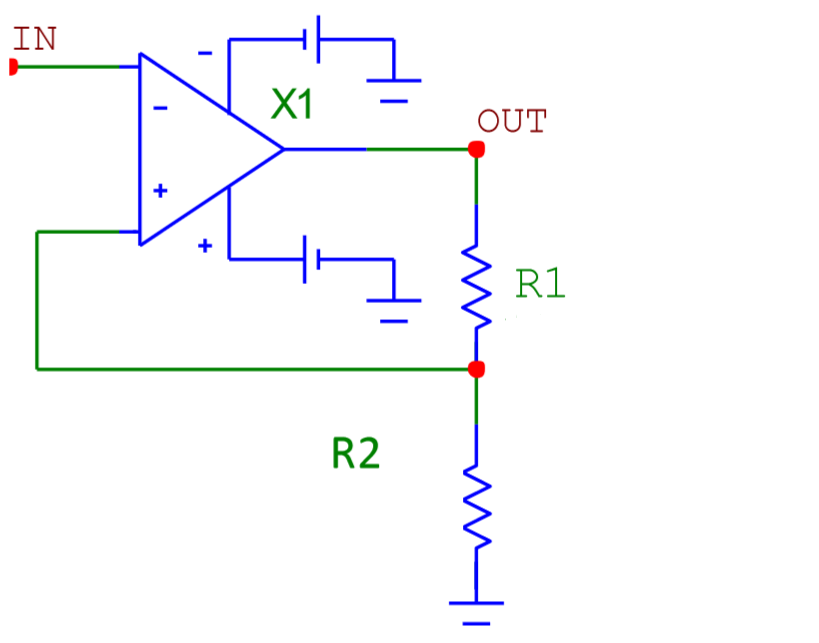
\includegraphics[scale=0.5]{triggerSchmitt.png}
\caption{ Trigger di Schmitt realizzato con un OpAmp modello TL081.\label{circuito3}}
\end{figure}

Questo circuito è un trigger di Schmitt, ovvero un circuito discriminatore con isteresi e reazione positiva.\\
Al circuito è stata inviata una tensione sinusoidale di ampiezza $V_S = /pm V$ a frequenza fissa $f = /pm Hz$, successivamente si sono misurate le tensioni in uscita nei due stati possibili del circuito: $V_{OH} = /pm V$ e $V_{OL} = /pm V$, dalle quali si sono ricavati i valori attesi per le tensioni di soglia $V_{1,ATT,TH}= -V_{OH}/(1+R_1/R_2)= /pm V$ e $V_{2,ATT,TH}= V_{OL}/(1+R_1/R_2) = /pm V$. Si sono poi misurate direttamente le tensioni $V_{1,TH}= /pm V$ e $V_{2,TH} = /pm V$ \rem{sono in accordo o no?!}.\\

\subsection*{2. Dipendenza dall'ampiezza e dalla frequenza e limiti del circuito}



\section*{D. Multivibratore astabile}
\subsection*{1. Analisi e montaggio del circuito}

Un circuito multivibratore astabile come quello in figura\ref{circuito4} può essere realizzato partendo dal trigger di Schmitt e inserendo componenti nuovi: una resistenza $R$, un condensatore $C$ e due diodi Zener.\\
\begin{figure}[h]
\centering
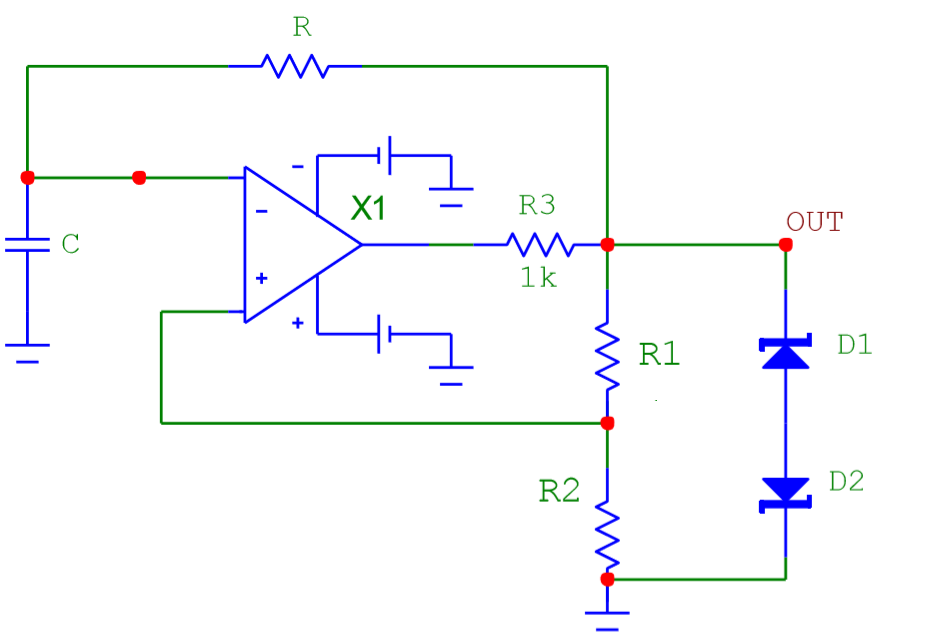
\includegraphics[scale=0.5]{multivibratoreAstabile.png}
\caption{Multivibratore asyabile realizzato con un OpAmp modello TL081.\label{circuito4}}
\end{figure}

Si è determinato il periodo di oscillazione in funzione degli elementi resistivi: 
\begin{center}
$T=2\tau\, log\left( 1\,+\,2\frac{R_2}{R_1}\right)$ 
\end{center}
Dunque per ottenere un periodo dell'onda quadra di $\sim 2ms$ si deve scegliere $\tau = RC\simeq 00\,ms$.
A questo punto abbiamo potuto montare il circuito con $R\,= /pm $, $C\,= /pm $, $R_1\,= /pm $, $R_2\,= /pm $ e $R_3\,= /pm $, con un' alimentazione per l'OpAmp di 15 V.\\

\subsection*{2. Verifica funzionamento del circuito}
\rem{punti 2 e 3 della scheda}\\




\subsection*{3. Dipendenza dalla tensione di alimentazione}


\subsection*{4. Limitazioni alla frequenza del segnale in ingresso}





 


\end{document}